\documentclass[12pt]{article}
\usepackage{background}
\usepackage{graphicx}
\usepackage[margin=1in]{geometry}
\usepackage{setspace}
\usepackage{hyperref}
\usepackage{xcolor}
\usepackage{tikz}
\usepackage{listings}
\usepackage{xcolor}
\usepackage{float}
\usepackage{subcaption}
\usepackage{circuitikz}
\usepackage[justification=centering]{caption}

\lstset{
	language=Python,
	backgroundcolor=\color{black!5},
	basicstyle=\ttfamily\small,
	breaklines=true,
	keywordstyle=\color{blue},
	commentstyle=\color{green},
	stringstyle=\color{red},
	identifierstyle=\color{black},
	morekeywords={def,class},
	morekeywords={import, as},
	frame=single,
	rulecolor=\color{black},
	tabsize=4,
	showstringspaces=false
}

\backgroundsetup{
	scale=0.5,
	color=black,
	opacity=0.1,
	angle=0,
	position=current page.center,
	vshift=-5cm,
	hshift=0cm,
	contents={
\includegraphics[width=\paperwidth, height=\paperheight]{figs/logo.jpg}}
}

\setcounter{secnumdepth}{2} % Enables numbering for sections and subsections
\setcounter{tocdepth}{2} % Includes subsections in the TOC

\title{\textbf{Multiplexed Seven-Segment Display Clock using Arduino and 7447 Decoder}}
\author{J.KEDARANANDA\\EE24BTECH11030}
\date{March 2025}

\begin{document}
	
	\maketitle
	\tableofcontents
	\newpage
	
	% --- Existing Content Starts Here ---
	
	\section{Introduction : }
	A seven-segment display (SSD) is widely used for displaying numerical data in digital clocks, calculators, and other embedded systems. To drive multiple SSDs efficiently, multiplexing is employed, where displays are activated sequentially at high speed to create a perception of continuous display. In this project, an Arduino Uno controls six common-anode SSDs via a 7447 decoder, using Boolean logic for digit selection and updating the clock time.
	
	\section{Hardware Components : }
	\begin{itemize}
		\item \textbf{Arduino Uno}: The main microcontroller handling the clock logic and multiplexing.
		\item \textbf{7447 BCD to 7-segment decoder}: Converts binary-coded decimal (BCD) signals from the Arduino into segment activation for the SSDs.
		\item \textbf{Six Common-Anode Seven-Segment Displays}: Used to display the time in HH:MM:SS format.
		\item \textbf{Push Buttons}: Three buttons for manual time adjustment (hours, minutes).
		\item \textbf{Resistors (220$\Omega$)}: Used to limit current to the display segments.
		\item \textbf{Jumper Wires and Breadboard}: Used for circuit connections.
	\end{itemize}
	
	\section{Circuit Connections : }
	\subsection{BCD Inputs for 7447 Decoder}
	The Arduino controls the BCD inputs of the 7447 decoder using the following pin mapping:
	\begin{table}[h]
		\centering
		\begin{tabular}{|c|c|}
			\hline
			\textbf{BCD Input} & \textbf{Arduino Pin} \\
			\hline
			A & D2 \\
			B & D3 \\
			C & D4 \\
			D & D5 \\
			\hline
		\end{tabular}
		\caption{BCD Input Connections}
	\end{table}
	\newpage
	\subsection{Seven-Segment Display (SSD) Common Pins for Multiplexing}
	Each SSD's common pin is connected to a dedicated Arduino digital pin for selective enabling during multiplexing:
	\begin{table}[h]
		\centering
		\begin{tabular}{|c|c|}
			\hline
			\textbf{SSD Position} & \textbf{Arduino Pin} \\
			\hline
			Hours Tens & D6 \\
			Hours Units & D7 \\
			Minutes Tens & D8 \\
			Minutes Units & D9 \\
			Seconds Tens & D10 \\
			Seconds Units & D11 \\
			\hline
		\end{tabular}
		\caption{SSD Common Pin Connections}
	\end{table}
	
	\section{Hardware Setup : }
	\subsection{Components Used}
	\begin{itemize}
		\item Arduino Uno
		\item Six Common Anode 7-segment displays
		\item One 7447 BCD to 7-segment decoder
		\item Jumper wires
		\item Breadboard
		\item 220-ohm resistors
	\end{itemize}
	\newpage
	\subsection{Circuit Connections}
	The following table outlines the connections between the Arduino, the 7447 decoder, and the SSDs:
	
	\begin{table}[h]
		\centering
		\caption{Pin Connections}
		\begin{tabular}{|c|c|c|}
			\hline
			Component & Arduino Pin & Purpose \\
			\hline
			7447 BCD A & D2 & BCD Input A \\
			7447 BCD B & D3 & BCD Input B \\
			7447 BCD C & D4 & BCD Input C \\
			7447 BCD D & D5 & BCD Input D \\
			\hline
			Hours Tens (COM) & D6 & Multiplexing Control \\
			Hours Units (COM) & D7 & Multiplexing Control \\
			Minutes Tens (COM) & D8 & Multiplexing Control \\
			Minutes Units (COM) & D9 & Multiplexing Control \\
			Seconds Tens (COM) & D10 & Multiplexing Control \\
			Seconds Units (COM) & D11 & Multiplexing Control \\
			\hline
		\end{tabular}
	\end{table}
	\subsection{Circuit Setup Steps}
	\textbf{Step 1:} Connecting the 7447 Decoder\newline
	Connect the BCD inputs (A, B, C, D) of the 7447 to the Arduino's digital pins D2 to D5.\newline
	\textbf{Step 2:} Connecting the 7-Segment Displays\newline
	Connect the common anode terminals of each SSD to the Arduino’s pins D6 to D11 for multiplexing control.\newline
	\textbf{Step 3:} Connecting Resistors\newline
	Use 220-ohm resistors between the 7447 outputs and the SSD segment inputs to limit current.\newline
	\textbf{Step 4:} Powering the Circuit\newline
	Connect the Arduino 5V and GND pins to the breadboard’s power rails to provide power to all components.\newline
	\subsection{Pin Labelling}
	\begin{figure}[h]
		\centering
		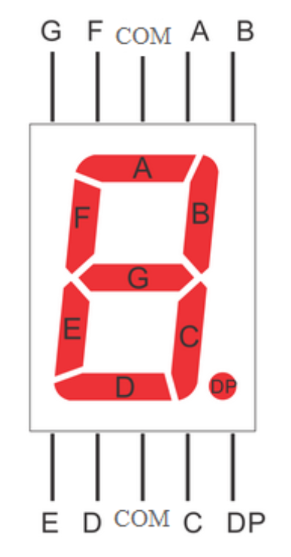
\includegraphics[width=0.2\textwidth]{figs/ssd.png}
	\end{figure}
	\begin{figure}[h]
		\centering
		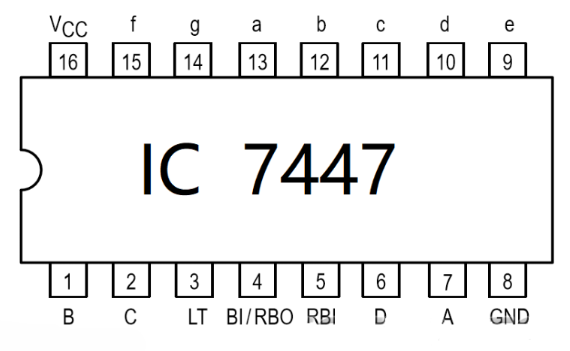
\includegraphics[width=0.4\textwidth]{figs/7447.png}
	\end{figure}
	\newpage
	\section{Final Setup : }
	\begin{figure}[h]
		\centering
		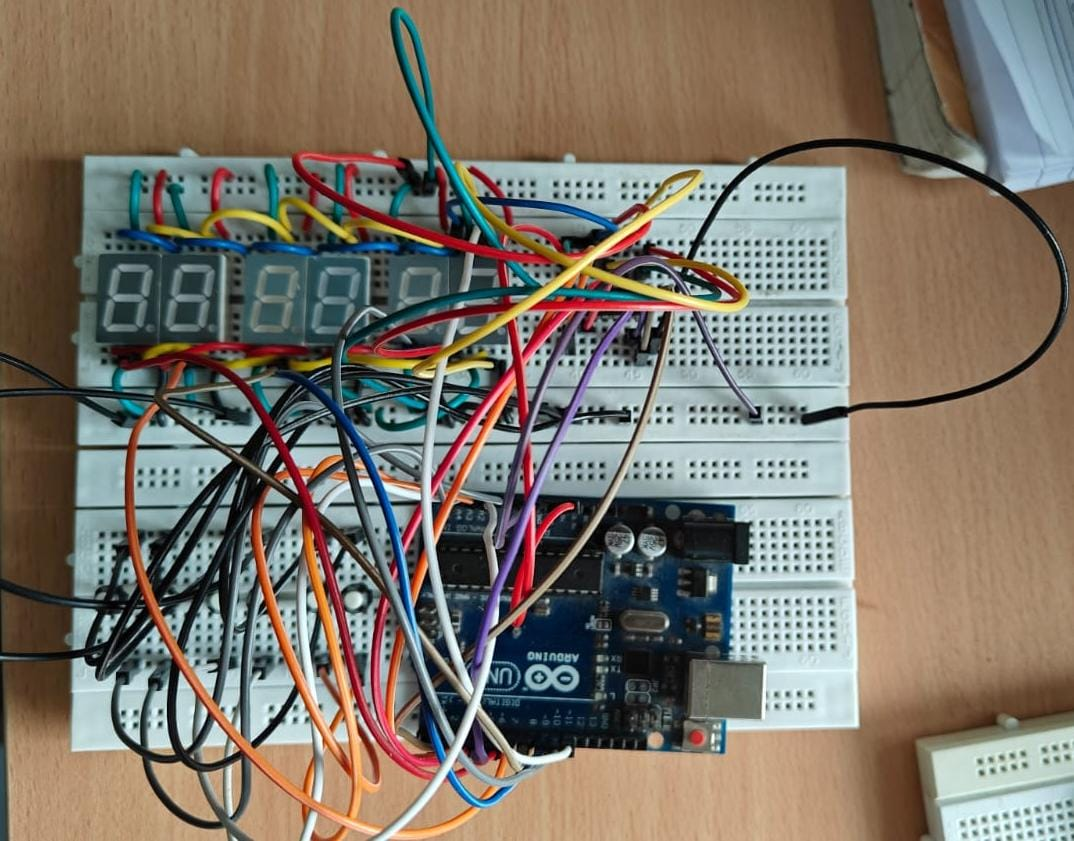
\includegraphics[width=0.4\textwidth]{figs/setup.png}
	\end{figure}
	\newpage
	\section{Working Principle : }
	\subsection*{Time Initialization}
	The clock starts at a predefined time when powered on. In this case, it is set to 12:00:00. Since the time is stored in Binary-Coded Decimal (BCD) format, the initial values are chosen accordingly:
	\begin{itemize}
		\item Hours: \textbf{0001 0010} (BCD for 12)
		\item Minutes: \textbf{0000 0000} (BCD for 00)
		\item Seconds: \textbf{0000 0000} (BCD for 00)
	\end{itemize}
	This initialization ensures that the clock starts at a consistent value every time it is powered on or reset. The BCD format allows for easy digit extraction when displaying the time on the seven-segment displays. Additionally, buttons are provided to manually adjust the hours and minutes.
	
	\subsection*{Displaying a Single Digit on the 7447 Decoder}
	The clock uses a 7447 BCD-to-seven-segment decoder to drive the display. To show a number, we must provide a corresponding Binary-Coded Decimal (BCD) input to the decoder. The decoder then activates the correct segments of the seven-segment display to form the digit. By controlling the four BCD input lines, any digit from 0 to 9 can be displayed. The key requirement is to ensure that only the required bits change while keeping the others stable, preventing unintended segment activations.
	
	\subsection*{Multiplexing the Display}
	Since the clock consists of six seven-segment displays but only one 7447 decoder is available, we use multiplexing to display all digits sequentially. Each digit is turned on for a brief moment before switching to the next, and this cycle repeats rapidly. This approach takes advantage of persistence of vision, where the human eye perceives all digits as being continuously lit. The multiplexing process involves:
	\begin{itemize}
		\item Extracting each digit from the time variables.
		\item Sending the corresponding BCD input to the 7447 decoder.
		\item Activating only one display at a time while keeping others off.
		\item Repeating this process in a continuous loop.
	\end{itemize}
	
	\subsection*{Timer1 Initialization}
	A precise timekeeping mechanism is necessary to maintain accuracy in the clock. Timer1 is configured to generate an interrupt every second, ensuring that the time updates correctly. This is achieved using a hardware timer, which operates independently of the main program execution. The timer is set in Clear Timer on Compare Match (CTC) mode, where it counts up to a predefined value and then resets. A prescaler is applied to slow down the counting speed, making it possible to achieve exactly one-second intervals.
	
	\subsection*{Timer1 ISR (Interrupt Service Routine)}
	The clock must update the displayed time every second without manual intervention. This is handled using an interrupt service routine (ISR) triggered by Timer1. Each time the interrupt occurs:
	\begin{itemize}
		\item The seconds counter increases by one.
		\item If the units place of seconds exceeds 9, it rolls over to the next tens place.
		\item Once seconds reach 60, they reset to zero, and minutes increase by one.
		\item The same logic applies to minutes and hours, ensuring a proper time progression.
		\item The hours reset to 1 after reaching 12 to maintain a 12-hour format.
	\end{itemize}
	Using a timer interrupt ensures that the clock keeps accurate time without being affected by other operations in the main program.
	
	
	\section{Conclusion : }
	This implementation provides a simple yet effective way to build a digital clock using BCD-based 7447 decoders and SSDs. The use of multiplexing optimizes the number of components, and timer interrupts ensure accurate timekeeping.
	
\end{document}

\end{document}
